
\documentclass[11pt]{article}
    \usepackage{pdfpages} 
  	\usepackage{ucs} 
	\usepackage[utf8x]{inputenc} % Включаем поддержку UTF8  
	\usepackage[russian]{babel}  % Включаем пакет для поддержки русского языка 
	\usepackage {mathtext}
	\usepackage{amsmath, amssymb}
	\usepackage{graphicx}
	\usepackage{listings}
	\usepackage{hyperref}
	\usepackage{revsymb}
	\usepackage{listings}
\lstset{language=[90]Fortran,
  basicstyle=\ttfamily,
  keywordstyle=\color{red},
  commentstyle=\color{green},
  morecomment=[l]{!\ }% Comment only with space after !
}
	\hypersetup{
    colorlinks=true,
    linkcolor=blue,
    filecolor=magenta,      
    urlcolor=cyan,
	}
	\urlstyle{same}
	\DeclareGraphicsExtensions{.pdf,.png,.jpg,.jpeg}
	\setcounter{MaxMatrixCols}{20}
	\graphicspath{{pictures/}}
    \title{\textbf{Подавление ферментативных систем биологических организмов ионизирующим излучением \\ -- \\ 
	Suppression of enzymatic systems of biological organisms by ionizing radiation}}
    \author{И.А.Юхновский, А.Г.Мелузов, А.В.Черемушкина}
    \date{сентябрь 2021}
    

\begin{document}
\maketitle
\thispagestyle{empty}
\section*{Аннотация}
Большая радиочувствительность ферментативных систем недостаточно изучена для случая теплового нейтронного излучения, что ограничивает наши полные знания о явлении. Значимое влияние данного вида ИИ связано с трансмутацией углеводородов в следствии заметной величины сечения поглощения нейтронов теплового спектра на этих уровнях энергий. В статье рассмотрена проблематика, теоретические основы радиационного подавления ферментативных систем, предложено понятие радиотропизма и рассмотрены варианты практического применения результатов исследований в области фармакологии.

\section*{Abstract}
The high radiosensitivity of enzymatic systems has not been sufficiently studied for the case of thermal neutron radiation, which limits our complete knowledge of the process. The significant influence of this type of ionizing radiation is associated with the transmutation of hydrocarbons as a result of the noticeable value of the neutron absorption cross section of the thermal spectrum at these energy levels. The article deals with the problems, theoretical foundations of radiation suppression of enzymatic systems, the concept of radiotropism is proposed and options for the practical application of the results of research in the field of pharmacology are considered.

\section{Введение}
Большая радиочувствительность ферментативных систем, катализирующих превращение триптофана в ауксин, в зеленых листьях растений была показана в серии работ Р.П.Вебера и С.А.Гордона в 50-ых годах ~\cite{GORDON}. 
Авторы показали, что малые дозы облучения (50-100р) уменьшали содержание ауксина в молодых растениях фасоли, а при инфильтрации триптофана в облученных листьях ауксина образуется меньше, чем в необлученных; экстракты из облученных листьев образуют in vitro меньше ауксина из триптофана, чем необлученные.

\begin{figure}[!htpb]
\centering
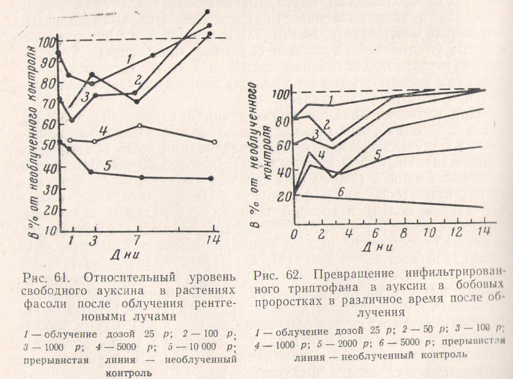
\includegraphics[scale=0.9]{kuzin}
\caption{Результаты исследований Р.П.Вебера и С.А.Гордона}
\label{}
\end{figure}

Гордон предполагает, что под влиянием облучения тормозится 
ферментативный процесс переходя индолацетальдегида в индолуксусную кислоту. Не описывая методов работы, автор утверждает, что в облученных листьях бобовых накапливается индолацетальдегид. Пири ~\cite{piri}, высказывая сомнения в методической части исследований с индолацетальдегидом, приходит к выводу, что еще не ясно, какой именно ферментативный процесс угнетается, но несомненным является факт подавления образования ауксина из триптофана в облученных листьях. 

Гордон показал, что подавляемая ферментативная система, находится в надосадочной жидкости, остающейся после удаления из гомогенатов ядер, пластид, митохондрий и микросом ~\cite{gordon_PinB}.

Исключительно большой интерес представляют исследования ферментативной активности отдельных органоидов клетки, так как наблюдаемые изменения активности могут быть непосредственно связаны с физико-химическим нарушением их субмикроскопической структуры. Наблюдения фундаментальной важности были сделаны по влиянию ионизирующей радиации на окислительное фосфорилирование в митохондриях клеток ~\cite{kuzin}.

При анализе разрушения фермента под влиянием ионизирующего излучения должны быть приняты к рассмотрению следующие возможности:

\begin{itemize} 
\item фермент разрушается под влиянием радиации; 
\item фермент выходит из пораженных клеток; 
\item фермент теряется вследствие смерти и лизиса ряда клеток;
\item фермент разрушается протеазами, освобождающимися под влиянием радиации;
\item фермент ингибируется образующимися или освобождающимися ингибиторами;
\end{itemize} 

Современные исследования проводятся для различных спектров ионизирующих излучений, однако публикаций о влиянии тепловых нейтронов на ферментативные системы нет. Изучение воздействия ионизирующего излучения (ИИ) на растения важно в связи с несколькими проблемами: 
\begin{itemize} 
\item наличие зон, в которых фоновая радиация - естественная или техногенная - повышена (повышение фона после проведения масштабных ядерных испытаний в прошлом веке); 
\item проблемы космической биологии; 
\item использование ИИ в сельскохозяйственной селекции;
\item общебиологические проблемы, связанные с фундаментальными закономерностями и особенностями воздействия ИИ на различные живые организмы.
\end{itemize} 

В ~\cite{Gudkov} рассмотрены первичные физико-химические реакции, индуцированные ИИ-излучением, которые включают образование различных форм активных форм кислорода (АФК) и являются причиной наблюдаемых изменений функциональной активности растений. В обзоре подчеркивается роль перекиси водорода, долгоживущей АФК, не только как повреждающего агента, но и как медиатора - универсального внутриклеточного мессенджера, обеспечивающего механизм передачи сигналов на большие расстояния. Высказано предположение, что ИИ влияет на физиологические процессы в основном за счет нарушения регуляции их активности. Нарушение, по-видимому, становится возможным из-за того, что существует перекрестное взаимодействие между различными сигнальными системами растений, такими как АФК, кальций, гормональная и электрическая системы. В результате как острого, так и хронического облучения повышение уровня АФК может влиять на активность широкого спектра физиологических процессов, регулируя их как на генетическом, так и на физиологическом уровнях. 

Физика рассматривает проблемы более узко, чем биоинженерия, и работа ~\cite{Gudkov} не учитывает влияние эндофитных организмов ~\cite{vasileva}, а также радиационно-индуцированные эффекты сторонних наблюдателей (RIBE) ~\cite{ribe}, однако
, данные эффекты также должны учитываться при моделировании динамики ферментативных систем.

При успешном построении модели прямого и косвенного влияния ионизирующего облучения на ферментативные системы для полного спектра можно будет сделать вывод о наличии такого явления как радиотрофизм.


\section{Влияние ИИ на биологически значимые вещества}
В связи со сложностью изоляции нейтронов теплового спектра от остальных сопутствующих видов ИИ работы по влиянию тепловых нейтронов на биологические объекты не проводились. 

Значимое влияние оказывают процессы:
\begin{itemize} 
\item действие на воду; 
\item образование перекисей; 
\item действие на простые белки и продукты распада;
\item действие на нуклеиновые кислоты, нуклеопротеины и другие сложные белки;
\item действие на углеводы;
\item действие на липиды;
\item действие на ферменты и витамины;
\end{itemize} 


\section{Влияние ИИ на состояние и обмен веществ в живой клетке и тканях}
Значимое влияние оказывают процессы:
\begin{itemize} 
\item влияние на активность ферментов; 
\item влияние на состояние и обмен нуклеопротеинов и нуклеиновых кислот; 
\item влияние на обмен белков;
\item влияние на углеводный обмен;
\item влияние на обмен липидов;
\item влияние на минеральный обмен;
\item действие на ферменты и витамины;
\end{itemize} 

В нашем случае есть в наличии тепловая колонна - прибор по созданию и контролю радиационного поля тепловых нейтронов. Первые эксперименты были проведены группой Сметанин, Гурьева, Андреев ~\cite{andreev} на семенах гороха.

Была получена зависимость - Рис.2
\begin{figure}[!htpb]
\centering
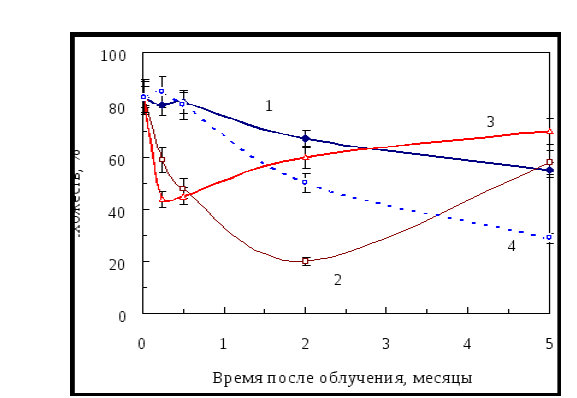
\includegraphics[scale=0.5]{goroh}
\caption{Всхожесть семян гороха (число нормальных проростков) в разные сроки после облучения в дозах 0 Гр (1), 190 мГр (2), 3 Гр (3) и 10 Гр (4). ~\cite{andreev}}
\label{}
\end{figure}

Там же были приведены параметры установки - Рис.3, Рис.4 и параметров установки - Рис.5
\begin{figure}[!htpb]
\centering
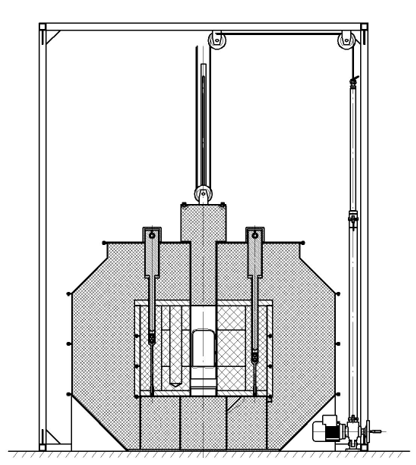
\includegraphics[scale=0.7]{ris_1}
\caption{Общая конструкция нейтронного конвертора ~\cite{andreev}}
\label{}
\end{figure}

\begin{figure}[!htpb]
\centering
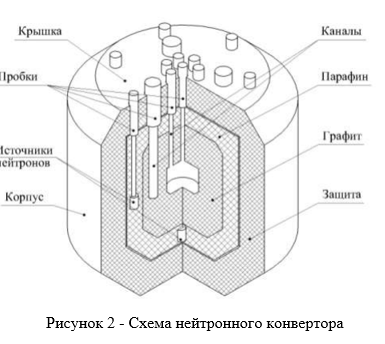
\includegraphics[scale=0.7]{ris_2}
\caption{Схема нейтронного конвертора ~\cite{andreev}}
\label{}
\end{figure}

\begin{figure}[!htpb]
\centering
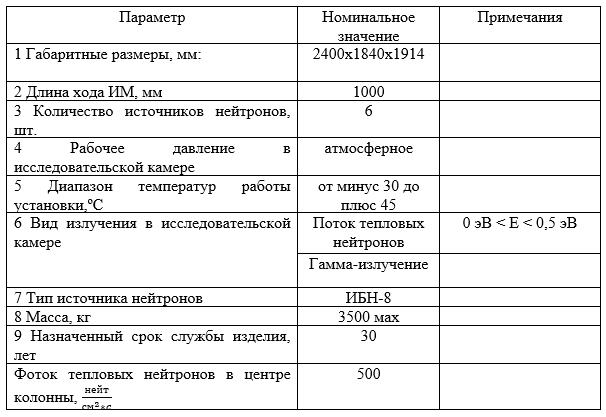
\includegraphics[scale=0.7]{tabl_1}
\caption{Основные технические характеристики нейтронного конвертора ~\cite{andreev_2}}
\label{}
\end{figure}

В результате экспериментов были получены выводы:
"Всхожесть семян, облученных в дозе 190 мГр, сначала постепенно уменьшалась в течение первых 2-х месяцев хранения, но к 5-ому месяцу восстановилась до уровня необлученных семян (рис. 23, кривая 2). После облучения семян в дозе 3 Гр она снижалась быстрее, но затем тоже восстанавливалась и через пять месяцев хранения всхожесть семян была даже выше исходной (кривая 3). Спустя две недели после облучения в дозе 10 Гр всхожесть семян, которая через неделю после облучения мало отличалась от всхожести необлученных семян, снижалась быстрее, чем всхожесть необлученных семян и после 5 месяцев хранения была вдвое ниже контрольной (кривая 4). 
То есть при хранении семян в зависимости от дозы облучения можно наблюдать разнонаправленные изменения всхожести. У семян, всхожесть которых была снижена ионизирующим облучением в малой дозе, происходит ее восстановление и даже некоторая стимуляция по сравнению с изменением всхожести необлученных семян. У семян, всхожесть которых или мало отличалась от исходной или была несколько повышенной после облучения в несколько больших дозах, при хранении, наблюдали только однонаправленное ее снижение по сравнению с контролем."~\cite{andreev_2}
Разнонаправленные изменения всхожести иллюстрируют сложность биологических процессов в горохе после облучения и зависимость от времени, что свидетельствует о наличии протекающих в это время в горохе биофизических и биохимических процессах. Повторение эксперимента должно дать отличие от полученных результатов в следствии отличия в микробиоме.

\section{Эндофитные организмы}
Повсеместное распространение эндофитных микроорганизмов является общепризнанным фактом, а открывающиеся возможности использования их в сельском хозяйстве вызывают огромный интерес к ним со стороны научного сообщества.В отличие от ризосферных (населяющих поверхность корней) и филлосферных (колонизирующих надземные органы) представителей растительно-микробного сообщества, эндофиты способны вступать с хозяином в более тесные взаимоотношения, в некоторых случаях сильно влияя на его фенотип и в целом принося определенную пользу, не формируя, однако, специфических структур, таких как клубеньки, в случае бобово-ризобиального симбиоза. Выполняя целый набор функций, среди которых модуляция уровней фитогормонов, продукция витаминов и улучшение снабжения
питательными веществами, эндофиты могут служить основой для биопрепаратов, что позволит в перспективе снизить необходимость использования минеральных удобрений в практике сельского хозяйства и вследствие этого негативное влияние последних на плодородие почв, биоразнообразие и здоровье человека. В этом обзоре рассмотрены такие аспекты растительно-эндофитного симбиоза, как биоразнообразие эндофитов бобовых и небобовых культур, экология данных микроорганизмов, вопросы их функциональной значимости, распространенные способы изучения, а также возможности их применения в сельском хозяйстве.~\cite{vasileva}
\subsection{Функции эндофитных бактений}
Ассоциации бактерий с растениями могли возникнуть и закрепиться в результате положительного отбора в пользу эндофитов ~\cite{v_85}.
Это предполагает наличие взаимовыгодного сотрудничества, и, действительно, при исследовании функциональной активности эндофитных штаммов оказалось, что ониоказывают положительное влияние на рост и развитие растительного организма, улучшают снабжение питательными веществами. Их присутствие положительно сказывается на устойчивости к стрессам различной природы, а кроме того, в ходе длительной коэволюции растений и эндофитов последние приобрели способность синтезировать химические соединения, первоначально производимые растением хозяином ~\cite{v_11, v_86}. В этом плане особого внимания заслуживает тот факт, что в стрессовых условиях повышается частота инфекции эндофитами ~\cite{v_17}.
Способность эндофитных микроорганизмов производить витамины и фитогормоны объясняет то, что заселенные эндофитами растения, как правило, более устойчивы к заболеваниям и дают высокие урожаи. Например, эндофиты Rahnella aquatilis и Pseudomonas putiida, способные синтезировать индолилуксусную кислоту, положительно влияют на рост и развитие некоторых злаков и редиса ~\cite{v_87}. Эндофит Bacillus subtilis, производящий гиббереллины, также положительно воздействует на растения ~\cite{v_88}.

\subsection{Разнообразие эндофитов гороха}
В горохе посевном были найдены Bacillus, Micromonospora, Ochrobactrum, Enterobacter, Pantoea, Pseudomonas, Serratia ~\cite{v_48, v_54, v_55, v_57, v_58}.

\subsection{Эндофитные микроорганизмы в сельском хозяйстве}
В практике традиционного сельского хозяйства самым распространенным, но также и самым энергоемким
является процесс получения минеральных удобрений, которые, при применении в высоких дозах, оказывают негативное влияние на здоровье человека, плодородие почв и биоразнообразие [22]. Хорошую альтернативу химическим удобрениям составляют микробиологические
препараты, применяемые в практике экологическиориентированного земледелия, подразумевающего использование устоявшихся симбиотических связей. Возможность использования микроорганизмов, населяющих внутренние ткани растений, для производства высокоэффективных биопрепаратов делает эту тему все более привлекательной для исследования. Существуют работы, демонстрирующие более высокую эффективность такого рода удобрений по сравнению с минеральными, в частности, в работе на штаммах Bacillus subtilis, полученных из борщевика, показано, что продуктивность
ярового ячменя (Hordeum vulgare L.) была выше, чем при использовании минеральных удобрений в рекомен дованной дозе [21]. Разработан ряд микробных препаратов на основе бактерий Azospirillum, Pseudomonas, Bacillus, Herbaspirillum, Acetobacter [19, 20]. Часто с их помощью удавалось даже избежать необходимости об работки пестицидами [20]. В опытах Гариповая и др. продемонстрировали целесообразность бактериальных обработок: болезненные проявления у обработанных штаммами Bacillus subtilis и Rhizobium leguminosarum растений фасоли были существенно снижены.

\subsection{Эндофитные микроорганизмы в поле ИИ}
Эндофитные организмы находятся в межклеточном пространмтве биологического организма и являются симбиотами, причем в различных пространственных координатах и временных отрезках их количественный и видовой состав будет отличаться. Этим обуславливается расхождения в экспериментальных данных при облучении биологических культур. События разрушения клетки передается между клетками и эндофитами сигнальными веществами. Так в ~\cite{Prise,Dong} приведены иллюстрации действия этого сигнального механизма.

\begin{figure}[!htpb]
\centering
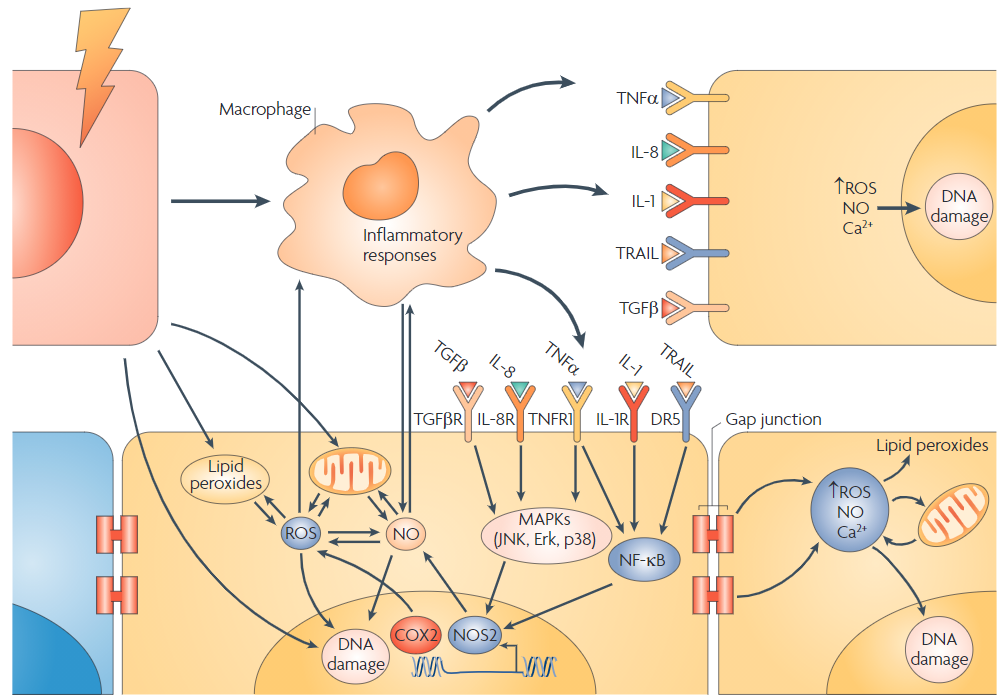
\includegraphics[scale=0.5]{ribe}
\caption{Основные пути воздействия на сигналы посторонних. Клетки реагируют на прямое излучение (эритроциты), вызывая реакции сторонних наблюдателей двумя ключевыми способами. Первый включает прямую межклеточную коммуникацию через щелевые контакты, а второй - высвобождение цитокиновых сигналов во внеклеточный матрикс. Не все ячейки отвечают (например, синяя ячейка). Invivo макрофаги могут быть важными медиаторами, которые в ответ на радиационно-индуцированное повреждение ткани испускают сторонние сигналы, влияющие на необлученные клетки (желтые клетки). Некоторые из ключевых путей и механизмов в настоящее время выясняются, включая роль в передаче сигналов, опосредованной цитокинами, в передаче сигнала через MAPK и ядерный фактор-kB (NF-kB) наряду с образованием активных форм кислорода и азота. COX2, циклооксигеназа2; DR5, рецептор смерти 5 (также известный как TNFRSF10B); ИЛ, интерлейкин; JNK, Jun N-терминальная киназа; NO, оксид азота; NOS2, NO-синтаза 2; АФК, активные формы кислорода; TGF $\beta$ , трансформирующий фактор роста-$\beta$; TGF$\beta$R, рецептор TGF$\beta$; TNF$\alpha$, фактор некроза опухоли-$\alpha$; TRAIL, TNF-родственный лиганд, индуцирующий апоптоз. ~\cite{Prise}}
\label{}
\end{figure}

\begin{figure}[!htpb]
\centering
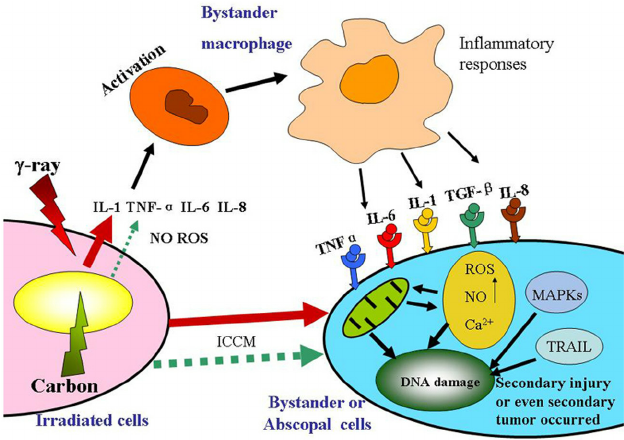
\includegraphics[scale=0.6]{ribe_1}
\caption{Роль промежуточных макрофагов во вторичном побочном эффекте, индуцированном радиацией. Когда опухолевые клетки облучали $\gamma$-лучами или ионами углерода, некоторые сигнальные факторы высвобождались для взаимодействия либо с вицинальными нормальными клетками, либо с макрофагами. Макрофаги могут быть активированы для генерации ряда цитокинов, чтобы дополнительно вызвать вторичный эффект свидетеля. ~\cite{Dong}}
\label{}
\end{figure}

Данный сигнальный механизм лежит в основе RIBE.

\section{RIBE - Radiation-Induced Bystander Effect}
В классических исследованиях радиационной биологии основное внимание уделялось ядерной ДНК как основной мишени радиационно-индуцированных повреждений. За последние два десятилетия это было оспорено значительным количеством научных данных, ясно показывающих, что радиационно-индуцированные сигнальные эффекты клеток играют важную роль в опосредовании общего радиобиологического ответа. Эти эффекты, обычно называемые радиационно-индуцированными эффектами сторонних наблюдателей (RIBE), бросают вызов традиционной теории ДНК-мишеней в радиационной биологии и подчеркивают важную роль клеток, не подвергающихся прямому проникновению радиации. ~\cite{ribe} Метод учитывает как присутствие соседних клеток ткани, так и наличие эндофитных организмов во внутриклеточном пространстве (микробиоме).

Иллюстрацией метода может служить ~\cite{Mariotti}, где изучались механизмы, регулирующие пути передачи вируса от посторонних лиц in vitro, сосредоточив внимание на нарушенной радиацией передаче сигналов (через интерлейкин 6, IL-6) облученных клеток после воздействия низких доз различных типов излучения.

Данные подтвердили важное влияние радиации на путь IL-6, ясно продемонстрировав решающую роль АФК (активных форм кислорода) в преобразовании эффекта начального радиационного воздействия и последующего длительного высвобождения IL-6. Более того, систематическое исследование зависимости дозы облучения / качества излучения, по-видимому, указывает на возрастающую эффективность облучения с высокой ЛПЭ (линейной передачей энергии) в высвобождении цитокина. Были проверены основные гипотезы о корреляции между прямым радиобиологическим повреждением и высвобождением сигнала и о цели излучения для этой конечной точки (секреция IL-6).

Результаты продемонстрировали роль активных форм кислорода и азота в сигнальных путях IL-6. Кроме того, принятый в исследовании системный подход радиационной биологии позволил  проверить и подтвердить гипотезы о поведении отдельной клетки при высвобождении цитокина после воздействия различных доз и различного качества ионизирующего излучения. 

Это значит, что определенный нами ранее список факторов влияющих на концентрацию фермента должен быть расширен пунктом - микробиом эндофитных организмов, поскольку, подвергаясь действию ИИ эндофиты по сигнальному механизму могут влиять на ферментативную систему. Учет этого параметра позволит объяснить воспроизводимость экспериментальных результатов на организмах из одного региона и на различия в данных на биологических организмах удаленных друг от друга как в пространстве, так и во времени.

\section{Радиотропизм}
Итак, были рассмотрены различные пути влияния ИИ на ферментативные системы и концентрацию биохимических веществ. Процесс, как мы видим, достаточно сложный и может быть зашумлен другими биологическим процессами, протекающими параллельно. 
Целесообразно рассмотреть более простую биологическую систему - растение.
В общем случае, мы можем говорить об особом виде тропизма - радиотропизме, как реакции растения в ответ на ИИ внешней среды.

В тропизме микроорганизмов у паразитов выражается в свойстве избирать в качестве среды обитания определённые организмы (видовой тропизм) или органы (органный, или тканевой, тропизм). Видовой тропизм обусловливает круг резервуаров и источников возбудителей инфекционных и паразитарных болезней, органный — место локализации возбудителя и специфического патологического процесса в организме хозяина.
Знания о тропизме используют при заборе материала для микробиологического исследования. Органный тропизм высоко выражен у вирусов, менее у облигатно-патогенных бактерий, мало — у условно-патогенных бактерий и грибов.



\subsection{Тропизмы}
Тропизм растений определяется ~\cite{dic_tropism} как ответные реакции растений на различные односторонние воздействия раздражителей внешней среды (свет, земное притяжение, химические вещества и др.) заключаются в направленных ростовых и сократительных движениях (изгибах) органов растения, приводящих к изменению его ориентации в пространстве. Ростовые движения зависят от вида раздражителя, механизм действия которого на растения сложен. Эти движения могут возникать в растущих частях растений, как следствие более быстрого роста клеток, расположенных на одной стороне органа растения (стебле, корне, листе). В органах растения возникают растяжения, связанные с асимметричным распределением в них фитогормонов роста растений — ауксина и абсцизовой кислоты и др.

Тропизмы растений различают в зависимости от вида раздражителя:

\begin{itemize} 
\item Геотропизм ~\cite{geo_tropism} - связан с воздействием на растения силы тяжести Земли. При положительном геотропизме рост главного корня направлен строго вниз по направлению к центру Земли, что связано не только с деятельностью гормонов, но и с особыми крахмальными зёрнами в корневом чехлике, выполняющим роль статолита. Отрицательный геотропизм характерен для главного стебля.
\item Фототропизм ~\cite{photo_tropism} - вызывает направленный изгиб растения к источнику света. Этот изгиб имеет химическую природу. Под влиянием фитогормона ауксина на теневой стороне деление и рост клеток интенсивнее по сравнению со световой стороной, где ауксина меньше и рост клеток замедлен. В связи с этим растение изгибается в сторону клеток медленно растущих, то есть к свету.
\item Хемотропизм - вызывает движение растений под влиянием химических соединений. Наиболее яркий пример хемотропизма — рост корней в сторону больших концентраций питательных веществ в почве.
\item термотропизмы - движение к теплу
\item гидротропизмы - движение к свету
\end{itemize} 

Для растений мы можем добавить радиотропизм - косвенное влияние на растений ИИ через угнетение ферментативных систем и прямое влияние - разложением биохимических элементов ответственных за рост (гетероауксина).

\subsection{Плохо объясняемые тропизмы у растений}
Некоторые встречающиеся тропизмы у деревьев сложно объяснимы. Они могут быть связаны с вирусным поражением растения, с механическим воздействием / повреждением. В простонародье скопления таких деревьев называют пьяный лес. Владимир Липаткин, декан факультета лесного хозяйства Московского государственного университета леса объясняет это явление следующим образом: "- Для учёных пьяные леса - вполне обычное и очень распространённое явление, описанное в учебниках по лесоводству ещё сотню лет назад. Они есть в каждом регионе. Даже в ближайшем Подмосковье можно встретить участки кривых деревьев. Есть такая зона в Алексеевской роще Лосиного Острова, есть участок в Приокско-террасном заповеднике Серпуховского района. Не надо искать мистику в «пьяных» лесах! Да, аномальность присутствует, но она заключается в том, что в определённый момент жизни дерева с ним что-то случилось. Например, появился вредитель (а их очень много: сосновый вертун, корневая губка и др.), который повредил точку роста и поспособствовал искривлению ствола. Или пронёсся сильный ураган, прошёл ледяной дождь. Всё это типы приспособления деревьев к жёстким условиям среды - не более того." ~\cite{lipatkin}
Это безусловно все так, однако, например, на Медведицкой гряде был замечен выход из недр радона во время продолжительного антициклона 19 июля 2015 г. ~\cite{petuhov} и как минимум было бы странно не обратить на этот факт внимание, так же, и как на аномалии в Чернобыле.

Странный лес расположен в Шиловском районе Рязанской обл. Как его только ни называют - ведьмин, дьявольский, пьяный, кривой… Все находящиеся на его территории сосны растут не так, как положено, - вверх, а почти у самого основания сначала сильно наклоняются к северу и только потом устремляются к небу. Есть деревья-арки, есть стволы, закрученные в бараний рог. «Аномальный участок занимает площадь примерно 1,5 км2, а за ним растут вполне нормальные сосновые боры с деревьями с ровными стволами. Этот же «пьяный» лес абсолютно мёрт­вый: молодняка там нет, ягод и грибов не найти даже в урожайный год.

«Танцующие» сосны рязанского «пьяного» соснового бор не единственные в России. Есть участок скрюченных деревьев недалеко от деревни Яреньга в Архангельской обл. Аномальная зона с искривлёнными сос­нами обнаружена поблизости от хутора Миасский под Челябинском. В Калининградской обл. на территории Куршской косы есть свой уникальный участок леса. Здесь его называют не ведьминым или пьяным, а танцующим. 

Основная часть кривых лесов - сосновые. Но есть и «пьяные» берёзовые рощи. В Лаишев­ском районе Татарстана берёзы сначала растут прямо, а потом делают боковой изгиб и опять продолжают расти вверх. Своя «пьяная» берёзовая роща есть в Хибинах на Кольском полуострове и на Медведицкой гряде на границе Саратовской и Волгоградской областей. 

«Медведицкая гряда находится на месте уникального тектонического разлома и считается одной из наиболее мощных аномальных зон России. Берёзы здесь изгибаются очень причудливо. Одни согнулись в виде дуги, другие превратились в спирали, третьи стелются по земле. Мы провели на Медведицкой гряде 11 экспедиций. Изучали радиацию, вредителей, экологические факторы - ничего нет. Но деревьям там неуютно и некомфортно - иначе бы их так не корёжило» Александр Петухов, замкоординатора «Космопоиска» ~\cite{lipatkin}

В двадцати километрах к северо-западу от  Хаффорда (в Саскачеване, Канада), и в пяти километрах к юго-западу от Алтикане, есть роща корявых осин. У деревьев резко закручены стволы и ветви, будто кто-то взял их в узлы.

\begin{figure}[!htpb]
\centering
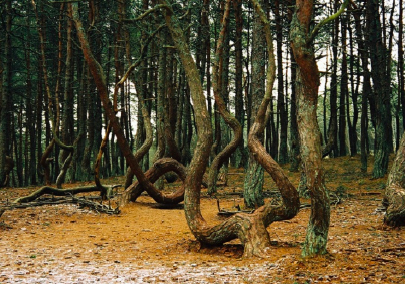
\includegraphics[scale=0.9]{chernobyl_1}
\caption{Рыжий лес в Чернобыле}
\label{}
\end{figure}


\begin{figure}[!htpb]
\centering
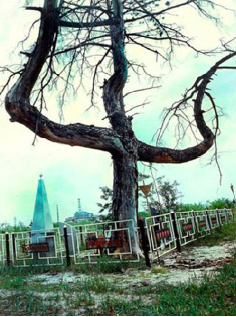
\includegraphics[scale=0.9]{chernobyl_2}
\caption{Дерево крест в Чернобыле}
\label{}
\end{figure}

\begin{figure}[!htpb]
\centering
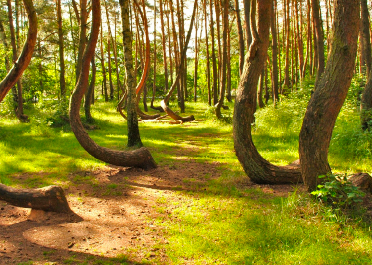
\includegraphics[scale=0.9]{gryfino_1}
\caption{Кривой лес в Польше Gryfino}
\label{}
\end{figure}

\begin{figure}[!htpb]
\centering
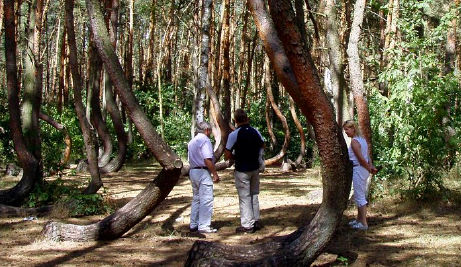
\includegraphics[scale=0.9]{gryfino_2}
\caption{Кривой лес в Польше Gryfino}
\label{}
\end{figure}

\begin{figure}[!htpb]
\centering
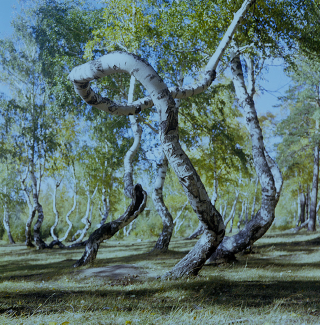
\includegraphics[scale=0.9]{medved}
\caption{Медведицкая гряда}
\label{}
\end{figure}

\begin{figure}[!htpb]
\centering
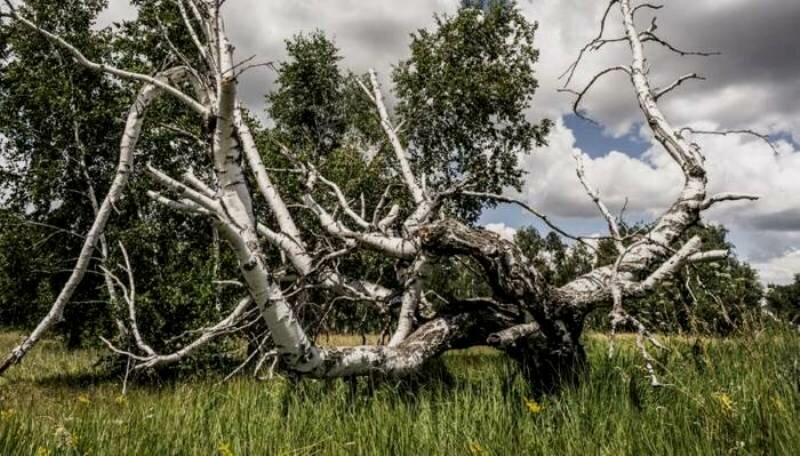
\includegraphics[scale=0.5]{medved_2}
\caption{Медведицкая гряда}
\label{}
\end{figure}



\begin{figure}[!htpb]
\centering
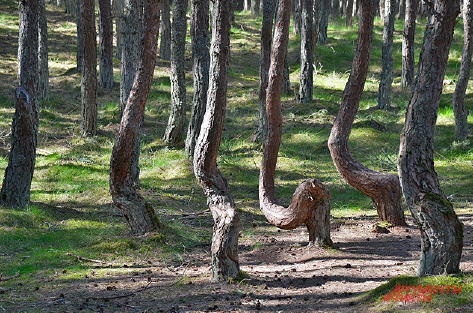
\includegraphics[scale=0.9]{Kurshskaya}
\caption{Куршская коса}
\label{}
\end{figure}

\begin{figure}[!htpb]
\centering
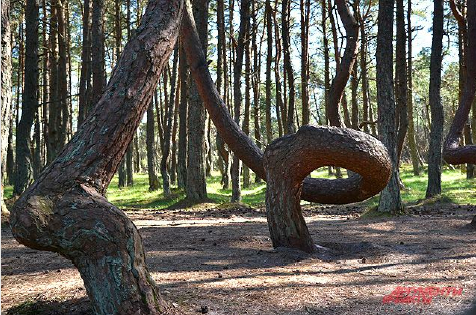
\includegraphics[scale=0.9]{Shilov}
\caption{Шиловский район Рязанской обл.}
\label{}
\end{figure}

\begin{figure}[!htpb]
\centering
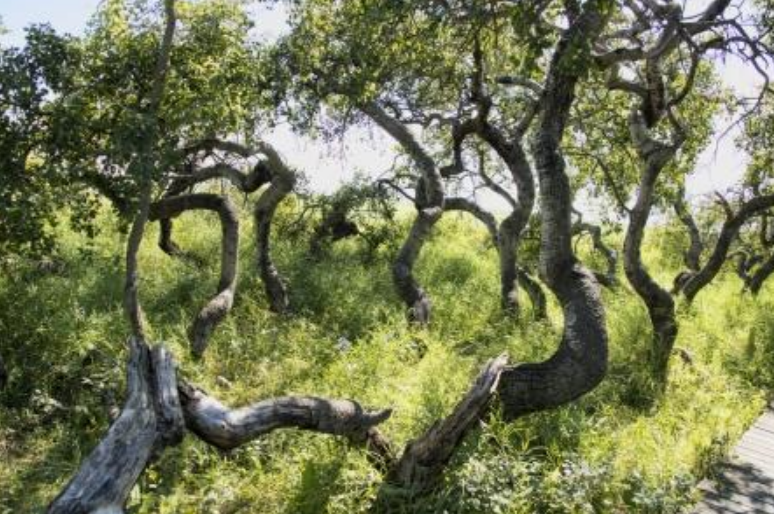
\includegraphics[scale=0.5]{Hoffard_1}
\caption{Роща корявых осиновых деревьев возле Хаффорда, Саскачеван, Канада}
\label{}
\end{figure}

\begin{figure}[!htpb]
\centering
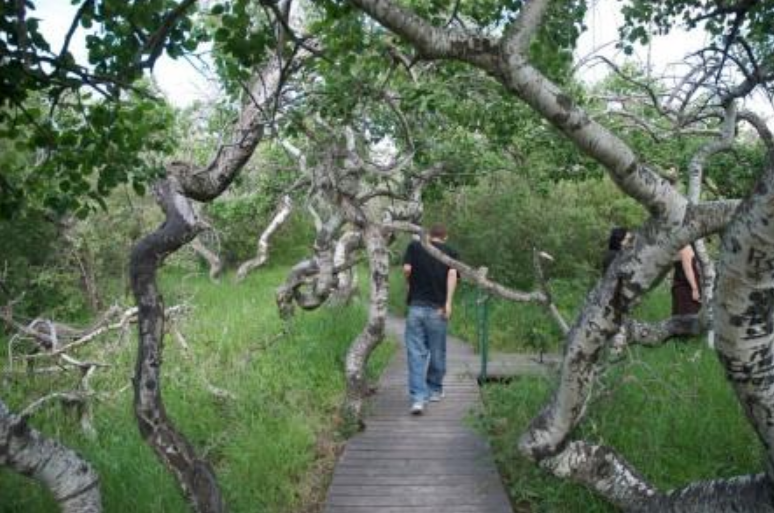
\includegraphics[scale=0.5]{Hoffard_2}
\caption{Роща корявых осиновых деревьев возле Хаффорда, Саскачеван, Канада}
\label{}
\end{figure}

\subsection{Радиотропизм для микроорганизмов}
Если говорить о радиотропизме для микрорганизмов, то можно наблюдать:
\begin{itemize} 
\item проявление в грибах - исследования Йокогамского национального университета с грибами ~\cite{hizh_12_11_2020}. Грибы "высасывают" из почвы радиоактивный цезий, но вот он остается на уровне грибницы и ножки. Вопрос - нет ли здесь влияние эндотрофов, которые "убираются" в своей среде, контролируют комфортные условия своего микробиома? Тогда по градиенту этдофитных микрооргаизмов мы сможем определить направление нахождения источника ИИ.

\item лягушки - Озерная лягушка Белоярского водохранилища, оно же охладитель Белоярской АЭС, накапливает долгоживущие радионуклиды в больших концентрациях, чем в контрольном водоеме; их концентрация у сеголеток и головастиков выше, а у взрослых особей не зависит от массы, пола и возраста ~\cite{bvv}. Вопрос, почему у взрослой лягушки не увеличивается концентрация радиоактивных элементов в организме по сравнению с анаэробной ("водной") стадией развития? Возможно у взрослой лягушки появляются процессы, которые блокируют поглощение радиоактивных металлов из окружающей среды? Могут ли это быть эндофиты?

\item рыбы - у рыбок Danio Rerio не наблюдается RIBE ~\cite{zebrafish_1,zebrafish_2,zebrafish_3,zebrafish_4,zebrafish_5}

\end{itemize} 

Всем этим явлениям мог бы дать объяснение радиотропизм.

Если попробовать найти радиотропизму микроорганизмов полезное применение, то можно рассмотреть вариант введения в биологический организм эндотрофов для снижения воздействия ИИ, например, при вынужденном нахождении в поле ИИ, при радиотерапии. В сельском хозяйстве - заселение эндотрофами выращиваемых растений на зараженной радионуклидами почве.

Химический путь такой радиационной деактивации эндофитами может быть проиллюстрирован использованием лиганда для связывания уранил-иона, открытого японскими учеными ~\cite{Keiko}


\begin{figure}[!htpb]
\centering
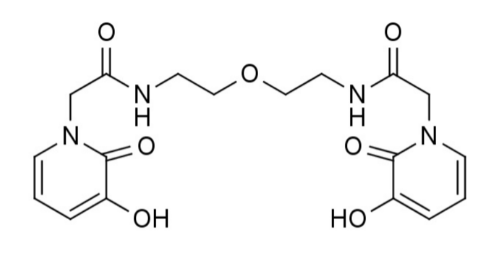
\includegraphics[scale=0.9]{ligand}
\caption{Гидроксипиридиновый лиганд 5LiO-1-Cm-3,2-hopo для связывания уранил-иона}
\label{}
\end{figure}

Еще одно перспективное направление - в статье ~\cite{gang} - приводятся исследования радикальной полимеризации в условиях окружающей среды при наличии молекулярного кислорода. Было показано, что факультативный электроген Shewanella oneidensis может контролировать катализируемую металлами живую радикальную полимеризацию в очевидных аэробных условиях (в то время как кислород является эффективным радикальным "тушителем"), сначала потребляя растворенный кислород посредством анаэробного дыхания, а затем направление внеклеточного электронного потока к металлическому катализатору. Результаты продемонстрировали способность Shewanella oneidensis использование кислорода и металлов для решения серьезных проблем синтеза полимеров. 

Можно ли использовать Shewanella oneidensis в качестве качественной реакции на присутствие урана и цезия в питательной среде? Что если подселить данную культуру в исследуемый организм лягушки? Будет ли концентрироваться цезий или уран внутри бактерии?

\begin{figure}[!htpb]
\centering
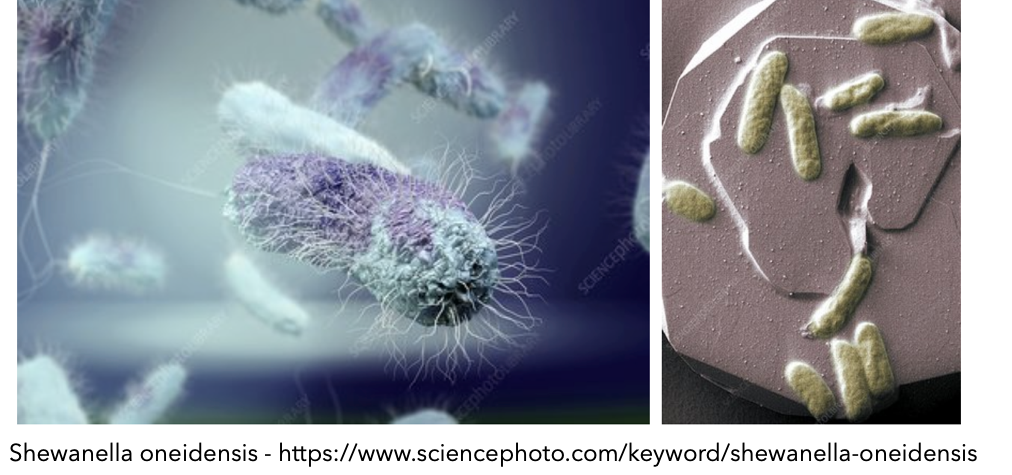
\includegraphics[scale=0.35]{shewanella}
\caption{Shewanella oneidensis}
\label{}
\end{figure}

\subsection{Классификация тропизмов}
Тропизмы классифицируются:

\begin{itemize} 
\item Ортотропизм — расположение органа растения вдоль градиента раздражителя; 
\item Диатропизм — расположение под прямым углом к градиенту раздражителя; 
\item Плагиотропизм — ориентация под любыми другими углами.
\end{itemize} 

В зависимости от природы ИИ могут наблюдаться различные типы. Так, например, для тепловых нейтронов - это будет плагиотропизм, из-за хаотичной разнонаправленной траектории частицы, а для высосоэнергетических спектров - ортотропизмы, ортотропизмы.

Причина, почему до сегодняшнего времени не было введено определение радиотропизма связано, как было указано ранее, с относительно гео-,фото-,хемо-тропизмов  слабым, в общем случае эффектом, однако все рассмотренные процессы указывают на его наличие и для аномальных случаев, при подтверждении отсутствия вирусного или механического воздействия, могут служить адекватным объяснением.

\section{Практическое значение}
Найти подтверждение влияния ИИ на ферментативные системы живых организмов мы можем косвенными методами при изучении рынка БАД: рост спроса на триптофан, теанин, глицин и рост спроса на микробиологические удобрения. Это может быть связано с ростом уровня естественного радиационного фона в следствии крупномасштабных ядерных испытаний в середине прошлого века, аварий на объектах атомной промышленности. При прочих равных условиях, при повышении радиационного фона ферментативные системы угнетаются, а значит, для продолжения нормального развития организма нужны компенсации в виде больших концентраций как ферментов, так и биохимических элементов участвующих в синтезе, что мы и наблюдаем на рынке в качестве повышения спроса.

\begin{figure}[!htpb]
\centering
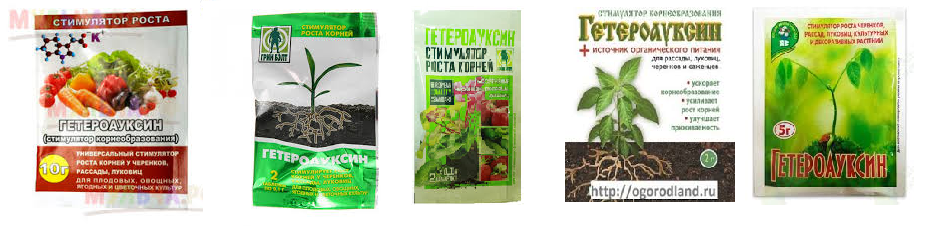
\includegraphics[scale=0.5]{geteroauxin}
\caption{Примеры продуктов на современном рынке удобрений}
\label{}
\end{figure}


\begin{figure}[!htpb]
\centering
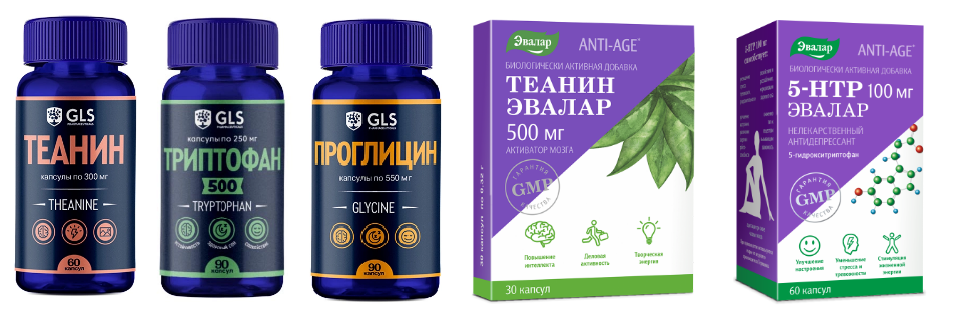
\includegraphics[scale=0.5]{products}
\caption{Примеры продуктов на современном рынке БАД}
\label{}
\end{figure}


\begin{figure}[!htpb]
\centering
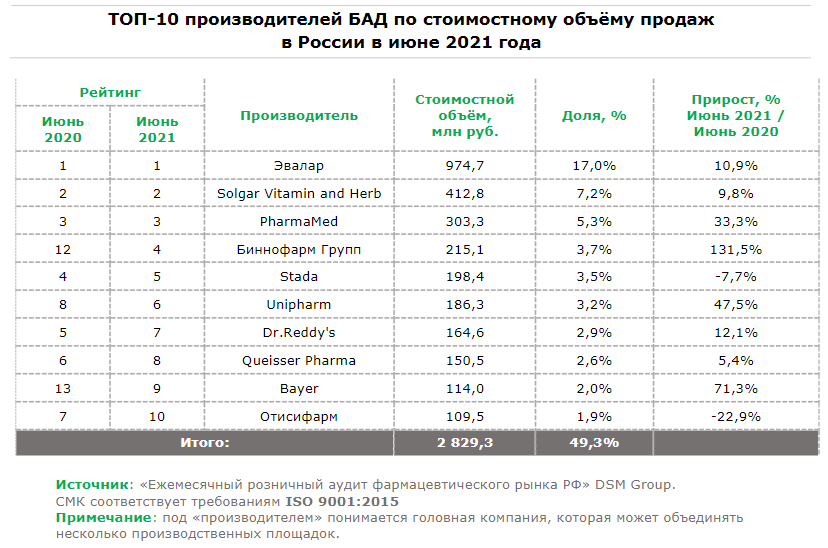
\includegraphics[scale=0.5]{bad}
\caption{ТОП-10 производителей БАД по стоимостному объёму продаж в России в июне 2021 года ~\cite{dsm}}
\label{}
\end{figure}

\subsection{Производство}
Производство препаратов может осуществляться:
\begin{itemize} 
\item химическим синтезом; 
\item химико-ферментативным синтезом; 
\item микробиологическим синтезом;
\end{itemize} 

Рассмотрим последний, на примере производства триптофана. 

В промышленном производстве L-триптофана обычно используются штаммы дрожжей Candida utilis, дефектные по aro-генам и, как следствие, ауксотрофные по фенилаланину и тирозину. Исходным сырьём обычно служит относительно дешёвая синтетическая антраниловая кислота, что является целесообразным по нескольким причинам. Во-первых, это упрощает и удешевляет процесс, а во-вторых, позволяет обойти механизмы регуляторного контроля (целевой продукт триптофан оказывает ингибирующее действие на антранилатсинтазу). В присутствии минимальных, не вызывающих регуляторных эффектов, количеств фенилаланина и тирозина мутанты Candida utilis переводит вводимую в культуральную среду антраниловую кислоту в L-триптофан.

Исходным сырьём в микробиологическом производстве триптофана может служить также синтетический индол. Процесс зависит от активности триптофан-синтазы и доступности серина.

Для описанных выше технологических процессов наши исследования будут полезны для улучшения выхода продукта путем снижения радиационного фона биологической защитой и методами биологической радиационной очистки компонентов, например, добавлением в производственный цикл агрегата водоподготовки для атомных станций. 

Кажущийся незначительный эффект малых доз радиации был продемонстрирован Фритц-Ниггли в  ~\cite{fnfritz_1, fnfritz_2}. Она показала, что состав внешней среды существенно изменяет радиочувствительность клеточных органелл. Автор повышала радиочувствительность метахондрий печени, помещая их в растворы маннита различной концентрации. После этого, облучение дозой в 50 р приводило к 30\%-ному подавлению окисления пировиноградной кислоты. При инкубации митохондрий в очень разбавленных растворах манита автору удавалось наблюдать снижение потребления кислорода на 60\% уже после облучения дозами в 0,1 р. 

Стокен сообщает ~\cite{stoken}, что тотальное облучение животных даже дозой в 100 р полностью прекращает фосфорилирование в ядрах клеток селезенки, тимуса, костного мозга и лимфатических узлов через час после облучения.

Угнетение окислительного фосфорилирования у микроорганизмов (дрожжи) было показано Мейселем ~\cite{meisel} , начиная с доз в 20000-30000 р., однако, исследования не были проведены для нейтронов в тепловом спектре, возвращаясь к теме нашей публикации, актуально изучить процесс на тепловых нейтронах. 

В исследованиях прошлого века зачастую присутствовала систематическая ошибка - игнорирование природы ИИ и энергетического спектра, в то время, как тепловые нейтроны могут трансмутировать отдельные атомы элементов органических соединений, тем самым разрушая не структурную, а химическую структуру органического соединения.

Вышеприведенные обоснования могут послужить основанием для проведения НИОКР с целю модернизации существующих технических процессов производства методом микробиологического синтеза на фармакологических предприятиях.

\subsection{Заключение}
Описанный в статье подход к изучению механизма подавления ферментативных систем имеет существенный недостаток в экспериментальной части, а именно - отсутствуют экспериментальные данные по нейтронам теплового спектра, который принципиально отличается от высокоэнергетических частиц тем,что кроме ионизации может вызывать процесс трансмутации ядер.

Теория RIBE, также как и исследования влияния эндофитных организмов на RIBE находятся в развитии и незавершены, поэтому вклад в развитие теории будет значительным при повторении ключевых экспериментов RIBE в области тепловых нейтронов.

Современное развитие программного обеспечения позволяет выполнить квантово-химические расчеты MOPAC, NWChem, ORCA, QUANTUM ESPRESSO~\cite{qe} , однако создание цифровой биологической модели является затруднительным из-за сложности квантово-механического описания биологической системы "группа клеток - эндофит", потому проведение экспериментальных исследований на текущий момент видятся безальтернативными, а начатые Андреевым В.В. эксперименты с горохом надо продолжить в рамках исследования RIBE с учетом эндофитных организмов гороха.

\begin{thebibliography}{3}

\bibitem{kuzin}
А.М.Кузин Радиационная Биохимия - Издательство Академии Наук СССР, Москва, 1962

\bibitem{GORDON}
GORDON SA. The effects of ionizing radiation on plants: biochemical and physiological aspects. Q Rev Biol. 1957 Mar;32(1):3-14. doi: 10.1086/401669. PMID: 13453658.

\bibitem{piri}
А.Пири В кн.: Ионизирующие излучения и клеточный метаболизм. М.1958, стр.73

\bibitem{gordon_PinB}
S.A.Gordon в кн.: "Progress in Radiobiol"., ed.J.S.Mitchell, Edinburgh, 1956, p.44


\bibitem{Gudkov}
Gudkov SV, Grinberg MA, Sukhov V, Vodeneev V. Effect of ionizing radiation on physiological and molecular processes in plants. J Environ Radioact. 2019 Jun;202:8-24. doi: 10.1016/j.jenvrad.2019.02.001. Epub 2019 Feb 15. PMID: 30772632.

\bibitem{vasileva} Васильева Е.Н., Ахтемова Г.А., Жуков В.А., Тихонович И.А. Эндофитные микроорганизмы в фундаментальных исследованиях и сельском хозяйстве // Экологическая генетика. - 2019. - Т. 17. - №1. - C. 19-32. doi: 10.17816/ecogen17119-32

\bibitem{ribe} Butterworth KT, McMahon SJ, Hounsell AR, O'Sullivan JM, Prise KM. Bystander signalling: exploring clinical relevance through new approaches and new models. Clin Oncol (R Coll Radiol). 2013 Oct;25(10):586-92. doi: 10.1016/j.clon.2013.06.005. Epub 2013 Jul 10. PMID: 23849503.

\bibitem{andreev}
Т.Р. СМЕТАНИН, Е.А. ГУРЬЕВА, В.В. АНДРЕЕВ ВЛИЯНИЕ НЕЙТРОННОГО ИЗЛУЧЕНИЯ МАЛОЙ МОЩНОСТИ НА РАЗВИТИЕ СЕМЯН ГОРОХА - Нижегородский государственный технический университет им. Р.Е. Алексеева

\bibitem{andreev_2}
В.В. Андреев Нейтронный конвертер как источник тепловых нейтронов - на правах рукописи

\bibitem{Mariotti} Mariotti LG, Bertolotti A, Ranza E, Babini G, Ottolenghi A. Investigation of the mechanisms underpinning IL-6 cytokine release in bystander responses: the roles of radiation dose, radiation quality and specific ROS/RNS scavengers. Int J Radiat Biol. 2012 Oct;88(10):751-62. doi: 10.3109/09553002.2012.703365. Epub 2012 Jul 24. PMID: 22709338.

\bibitem{v_85}
Thrall PH, Hochberg ME, Burdon JJ, Bever JD. Coevolution of symbiotic mutualists and parasites in a community context. Trends Ecol Evol. 2007;22(3):120-6. https://doi/org/10.1016/j.tree.2006.11.007.

\bibitem{v_17}
Zhang HW, Song YC, Tan RX. Biology and chemistry
of endophytes. Nat Prod Rep. 2006;23(5):753-771.
https://doi/org/10.1039/b609472b.

\bibitem{v_11}
Santoyo G, Moreno-Hagelsieb G, Orozco-Mosqueda
Mdel C, Glick BR. Plant growth-promoting bacterial
endophytes. Microbiol Res. 2016;183:92-99. https://
doi/org/10.1016/j.micres.2015.11.008.

\bibitem{v_86}
Malfanova N, Lugtenberg BJJ, Berg G. Bacterial
endophytes: who and where, and what are they doing
there? In: Molecular Microbial Ecology of the
Rhizosphere. Vol. 1. Ed. by F.J. de Bruijn. Hoboken:
John Wiley \& Sons, Ltd.; 2013. https://doi/
org/10.1002/9781118297674.ch36.


\bibitem{v_87}
Malfanova N, Lugtenberg BJJ, Berg G. Bacterial
endophytes: who and where, and what are they doing
there? In: Molecular Microbial Ecology of the
Rhizosphere. Vol. 1. Ed. by F.J. de Bruijn. Hoboken:
John Wiley \& Sons, Ltd.; 2013. https://doi/org/10.1002/9781118297674.ch36.


\bibitem{v_88}
Malfanova N, Kamilova F, Validov S, et al. Characterization
of Bacillus subtilis HC8, a novel plantbeneficial
endophytic strain from giant hogweed. Microb
Biotechnol. 2011;4(4):523-532. https://doi/org/10.1111/j.1751-7915.2011.00253.x.

\bibitem{v_48}
Elvira-Recuenco M, van Vuurde JW. Natural incidence of endophytic bacteria in pea cultivars under field conditions. Can J Microbiol 2000;46(11):1036-1041.
https://doi/org/10.1139/w00-098

\bibitem{v_54}
Tariq M, Hameed S, Yasmeen T, Ali A. Non-rhizobial
bacteria for improved nodulation and grain yield
of mung bean [Vigna radiata (L.) Wilczek]. Afr
J Biotechnol 2012;11:15012-15019. https://doi/org/10.5897/AJB11.3438.

\bibitem{v_55}
Гарипова С.Р., Гарифуллина Д.В., Маркова О.В.,
и др. Комплексная биологическая активность in
vitro эндофитных бактерий, выделенных из клубеньков гороха и фасоли // Известия Уфимского научного центра Российской академии наук. – 2015. –
№ 4–1. – С. 25–28. [Garipova SR, Garifullina DV,
Markova OV, et al. Complex biological activity in vitro
of endophytic bacteria isolated from pea and bean nodules.
Izvestiya Ufimskogo Nauchnogo Tsentra Rossiyskoy
Akademii Nauk. 2015;(4-1):25-28. (In Russ.)]

\bibitem{v_57}
Carro L, Sproer C, Alonso P, Trujillo ME. Diversity of
Micromonospora strains isolated from nitrogen fixing
nodules and rhizosphere of Pisum sativum analyzed
by multilocus sequence analysis. Syst Appl Microbiol.
2012;35(2):73-80. https://doi/org/10.1016/j.syapm.
2011.11.003.

\bibitem{v_58}
Carro L, Riesco R, Sproer C, Trujillo ME. Micromonospora luteifusca sp. nov. isolated from cultivated Pisum sativum. Syst Appl Microbiol. 2016;39(4):237-42.
https://doi/org/10.1016/j.syapm.2016.04.003

\bibitem{Prise}
Prise, K. and J. O’Sullivan. “Radiation-induced bystander signalling in cancer therapy.” Nature Reviews Cancer 9 (2009): 351-360.

\bibitem{Dong}
Dong, Chen \& He, Mingyuan \& Wenzhi, Tu \& Konishi, Teruaki \& Liu, Weili \& Xie, Yuexia \& Dang, Bingrong \& Li, Wenjian \& Uchihori, Yukio \& Hei, Tom \& Shao, Chunlin. (2015). The differential role of human macrophage in triggering secondary bystander effects after either gamma-ray or carbon beam irradiation. Cancer letters. 363. 10.1016/j.canlet.2015.04.013. 

\bibitem{dic_tropism}
~\url{https://dic.academic.ru/dic.nsf/ruwiki/304332}

\bibitem{geo_tropism}
~\url{https://dic.academic.ru/dic.nsf/ruwiki/248435}

\bibitem{photo_tropism}
~\url{https://dic.academic.ru/dic.nsf/ruwiki/1342106}

\bibitem{photo_tropism}
~\url{https://dic.academic.ru/dic.nsf/ruwiki/1342106}

\bibitem{hizh_12_11_2020}
"Химия и жизнь" стр.12, №11, 2020

\bibitem{zebrafish_1}
Choi VW, Yu KN. Embryos of the zebrafish Danio rerio in studies of non-targeted effects of ionizing radiation. Cancer Lett. 2015 Jan 1;356(1):91-104. doi: 10.1016/j.canlet.2013.10.020. Epub 2013 Oct 28. PMID: 24176822.

\bibitem{zebrafish_2}
Hatzi VI, Laskaratou DA, Mavragani IV, Nikitaki Z, Mangelis A, Panayiotidis MI, Pantelias GE, Terzoudi GI, Georgakilas AG. Non-targeted radiation effects in vivo: a critical glance of the future in radiobiology. Cancer Lett. 2015 Jan 1;356(1):34-42. doi: 10.1016/j.canlet.2013.11.018. Epub 2013 Dec 13. PMID: 24333869.

\bibitem{zebrafish_3}
Kong EY, Choi VW, Cheng SH, Yu KN. Some properties of the signals involved in unirradiated zebrafish embryos rescuing $\alpha$-particle irradiated zebrafish embryos. Int J Radiat Biol. 2014 Dec;90(12):1133-42. doi: 10.3109/09553002.2014.932031. PMID: 24913297.

\bibitem{zebrafish_4}
Choi VW, Wong MY, Cheng SH, Yu KN. Effects of exogenous carbon monoxide on radiation-induced bystander effect in zebrafish embryos in vivo. Appl Radiat Isot. 2012 Jul;70(7):1075-9. doi: 10.1016/j.apradiso.2011.11.018. Epub 2011 Nov 18. PMID: 22119559.

\bibitem{zebrafish_5}
Bobe J, Goetz FW. Molecular cloning and expression of a TNF receptor and two TNF ligands in the fish ovary. Comp Biochem Physiol B Biochem Mol Biol. 2001 Jun;129(2-3):475-81. doi: 10.1016/s1096-4959(01)00353-0. PMID: 11399482.

\bibitem{bvv}
"Биология внутренних вод", 2020, 613-619 

\bibitem{Keiko}
Keiko Tagami, Shiego Uchida, Michael D.Wood \& Nicolas A. Beresford Radiocaesium transfer and radiation exposure of frogs in Fukusima prefecture

\bibitem{gang} 
Gang Fan, Austin J.Graham, Jayaker Kolli, Nathaniel A.Lynd and Benjamin K.Keitz "Aerobic radical polymerization mediated by microbial metabolism" (DOI: 10.1038/s41557-020-0460-1) 
 
\bibitem{lipatkin}
~\url{https://aif.ru/society/nature/pyanye_lesa_kakaya_nevedomaya_sila_skrutila_derevya}
 
\bibitem{petuhov}
~\url{https://www.youtube.com/watch?v=Yqzd2PYiUHk&lc=UgzHigNcDgq4GsQpiLN4AaABAg.9JRX0muIbRa9JkkkmnIBdY&ab_channel=UnionKOSMOPOISK}


\bibitem{dsm}
~\url{https://dsm.ru/upload/iblock/44c/44c18b8d692bb3679e608dd24890a85e.pdf}

\bibitem{fnfritz_1} 
H.Fritz-Niggli.Naturwissenschaften, 42, 85, 1955 

\bibitem{fnfritz_2} 
H.Fritz-Niggli.Naturwissenschaften, 43, 112, 425, 1956

\bibitem{stoken}
L.A.Stocken Radiation Res., Suppl. 1, 53, 1959

\bibitem{meisel} 
М.Н.Мейсель. В сб.: Действие облучения на организм - Изд-во АН СССР, 1955, стр.78

\bibitem{qe}
~\url{https://www.chemie.uni-bonn.de/pctc/mulliken-center/orca}

\bibitem{qe}
~\url{http://www.quantum-espresso.org/}

\end{thebibliography}

\end{document}